% 2021-08-23 revised by Banbara
\documentclass[dvipdfmx]{beamer}

%\usepackage{bxdpx-beamer}% dvipdfmxなので必要
\usepackage{listings,jlisting} %ソースコード貼り付けのため
\usepackage{tikz}
\usetikzlibrary{positioning}
\usetikzlibrary{shadows}
%\AtBeginDvi{\special{pdf:tounicode 90ms-RKSJ-UCS2}} % しおりが文字化けしないように

\usepackage{otf}
\usepackage{txfonts} % 数式・英文ローマン体を Lxfont にする
\renewcommand{\kanjifamilydefault}{\gtdefault}
\usepackage{graphicx,xcolor} % 文字の色

\usetheme{Warsaw}
%\usetheme{Darmstadt}
\setbeamertemplate{navigation symbols}{} % 右下のアイコンを消す
\setbeamertemplate{footline}[frame number] % スライド下のバーを消してフレーム番号を表示
\useoutertheme{shadow}                 % 箱に影をつける
\usefonttheme{professionalfonts}       % 数式の文字を通常の LaTeX と同じにする

%%%%%%%%%%%%%%%%%%%%%%%%%%%%%%%%%%%%%%%%%%%%%%%%%%%%%%%%%%%%%%%%
% User-defined Macro
%%%%%%%%%%%%%%%%%%%%%%%%%%%%%%%%%%%%%%%%%%%%%%%%%%%%%%%%%%%%%%%%
\newcommand{\compress}{\itemsep0pt\parsep0pt\parskip0pt\partopsep0pt}
% \newcommand{\compress}{\itemsep1pt plus1pt\parsep0pt\parskip0pt}
% \newcommand{\code}[1]{\lstinline[basicstyle=\ttfamily]{#1}}
\newcommand{\gringo}{\textit{gringo}}
\newcommand{\clasp}{\textit{clasp}}
\newcommand{\clingo}{\textit{clingo}}
\newcommand{\teaspoon}{\textit{teaspoon}}
\newcommand{\sat}{\textsf{SAT}}
\newcommand{\unsat}{\textsf{UNSAT}}
% \newcommand{\web}[2]{\href{#1}{#2\ \raisebox{-0.15ex}{\beamergotobutton{Web}}}}
% \newcommand{\doi}[2]{\href{#1}{#2\ \raisebox{-0.15ex}{\beamergotobutton{DOI}}}}
% \newcommand{\weblink}[1]{\web{#1}{#1}}
% \newcommand{\imp}{\mathrel{\Rightarrow}}
% \newcommand{\Iff}{\mathrel{\Leftrightarrow}}
% \newcommand{\mybox}[1]{\fbox{\rule[.2cm]{0cm}{0cm}\mbox{${#1}$}}}
% \newcommand{\mycbox}[2]{\tikz[baseline]\node[fill=#1!10,anchor=base,rounded corners=2pt] () {#2};}
% \newcommand{\naf}[1]{\ensuremath{{\sim\!\!{#1}}}}
% \newcommand{\head}[1]{\ensuremath{\mathit{head}(#1)}}
% \newcommand{\body}[1]{\ensuremath{\mathit{body}(#1)}}
% \newcommand{\atom}[1]{\ensuremath{\mathit{atom}(#1)}}
% \newcommand{\poslits}[1]{\ensuremath{{#1}^+}}
% \newcommand{\neglits}[1]{\ensuremath{{#1}^-}}
% \newcommand{\pbody}[1]{\poslits{\body{#1}}}
% \newcommand{\nbody}[1]{\neglits{\body{#1}}}
% \newcommand{\Cn}[1]{\ensuremath{\mathit{Cn}(#1)}}
% \newcommand{\reduct}[2]{\ensuremath{#1^{#2}}}
% \newcommand{\OK}{\mbox{\textcolor{green}{\Pisymbol{pzd}{52}}}}
% \newcommand{\KO}{\mbox{\textcolor{red}{\Pisymbol{pzd}{56}}}}
% \newcommand{\code}[1]{\lstinline[basicstyle=\ttfamily]{#1}}
% \newcommand{\lw}[1]{\smash{\lower2.ex\hbox{#1}}}
\newcommand{\llw}[1]{\smash{\lower3.ex\hbox{#1}}}

\newenvironment{tableC}{%
  \scriptsize
  \renewcommand{\arraystretch}{0.9}
  \tabcolsep = 0.6mm
  % \begin{tabular}[t]{p{6mm}|rlr|rlr|rlr|rlr|rlr}\hline
  %   \multicolumn{1}{l|}{\llw{問題   }} &
  \begin{tabular}[t]{l|rlr|rlr|rlr|rlr|rlr}\hline
    \multicolumn{1}{l|}{\llw{問題}} &
    \multicolumn{3}{c|}{UD1} &
    \multicolumn{3}{c|}{UD2} &
    \multicolumn{3}{c|}{UD3} &
    \multicolumn{3}{c|}{UD4} &
    \multicolumn{3}{c}{UD5} \\
    & 
    \multicolumn{1}{c}{既知の} & & \multicolumn{1}{c|}{ASP} & 
    \multicolumn{1}{c}{既知の} & & \multicolumn{1}{c|}{ASP} & 
    \multicolumn{1}{c}{既知の} & & \multicolumn{1}{c|}{ASP} & 
    \multicolumn{1}{c}{既知の} & & \multicolumn{1}{c|}{ASP} & 
    \multicolumn{1}{c}{既知の} & & \multicolumn{1}{c}{ASP} \\
    & 
    ベスト & &  & 
    ベスト & &  & 
    ベスト & &  & 
    ベスト & &  & 
    ベスト & &  \\
    \hline
  }{%
    \hline
  \end{tabular}
}
 % 自分用のマクロ

\title{解集合プログラミングを用いた\\ハミルトン閉路問題の解法に関する考察}
\author{平手 貴大\inst{1}\and  宋 剛秀\inst{2}\and 田村 直之\inst{2}\and 番原 睦則\inst{1}}
\date{日本ソフトウェア科学会第38回大会 (JSSST-2021)}
\institute{\inst{1}名古屋大学 大学院情報学研究科 \and \inst{2}神戸大学 情報基盤センター}

\begin{document}
%%%%%%%%%%%%%%%%%%%%%%%%%%%%%%%%%%%%%%%%%%%%%%%%%%%%%%%%%%%%%%%%%%%
\frame{\maketitle}
%%%%%%%%%%%%%%%%%%%%%%%%%%%%%%%%%%%%%%%%%%%%%%%%%%%%%%%%%%%%%%%%%%%
\begin{frame}{ハミルトン閉路問題(Hamiltonian Cycle Problem; HCP)}
  \begin{itemize}
  \item \alert{ハミルトン閉路問題}
    \begin{itemize}
    \item 与えられたグラフの全頂点をちょうど一度ずつ
      通る閉路が存在するかどうかを判定する問題である.
    \item 始点と終点が一致するという閉路の条件を
      取り除けば,ハミルトン路問題となる.
    \end{itemize}
  \item \alert{最短ハミルトン閉路問題}
    \begin{itemize}
    \item グラフの辺に距離が付随しているときに,
      最短距離のハミルトン閉路を求める問題である.
    \end{itemize}
  \item \alert{コスト制約付きハミルトン閉路問題}
    \begin{itemize}
    \item ハミルトン閉路問題に,距離の総和が所与の閾値以下
      (または以上)であることを制約条件として付加した問題である.
    \item 最近,二分決定グラフを用いた解の高速列挙アルゴリズムが提案されている~[湊+, 2020].
    \end{itemize}
  \end{itemize}
  \begin{alertblock}{}
    本研究では,無向グラフ上のハミルトン閉路問題
    およびその関連問題を対象とする.    
  \end{alertblock}
\end{frame}
%%%%%%%%%%%%%%%%%%%%%%%%%%%%%%%%%%%%%%%%%%%%%%%%%%%%%%%%%%%%%%%%%%%
\begin{frame}{コスト制約付きハミルトン路問題}
%%%%%%%%%%%%%%%%%%%%%%%%%%%%%%%%%%%%%%%%%%%%%%%
\begin{center}
  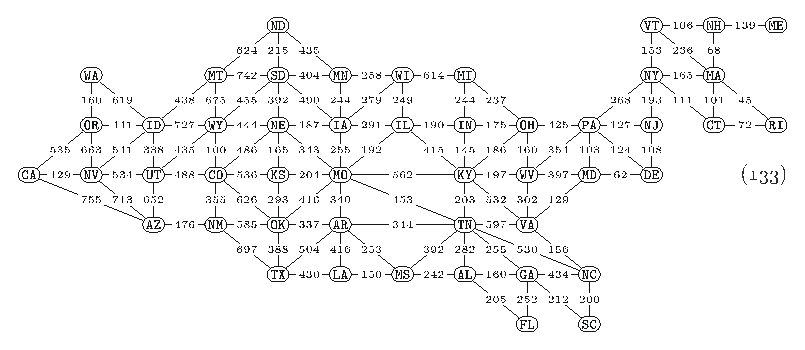
\includegraphics[width=0.8\linewidth]{fig/taocp_vol4fasc1b_p52_eq133.pdf}
\end{center}
\vfill
\only<1>{
\begin{itemize}
\item Knuth の The Art of Computer Programming に記載されている米国本
  土48州の隣接関係を表すグラフ
\item 頂点数は48,辺の数は105
\item 各辺に付与されている数字は州都の間の距離 (マイル)
\end{itemize}
}
\only<2>{
\begin{exampleblock}{}
  西海岸ワシントン州 (WA) から 東海岸メーン州 (ME) までの距離の総和
  がある閾値以下であるハミルトン路を求める問題を考える.
\end{exampleblock}
\begin{itemize}
\item WA から ME までのハミルトン路は 6,876,928 通りあり,
  最短ハミルトン路は 11,698 マイルである.
\item 閾値を最短距離の 10\%増 (12,868 マイル) とした場合,
  解の総数は 16,180 個ある.
\end{itemize}
}
\end{frame}
%%%%%%%%%%%%%%%%%%%%%%%%%%%%%%%%%%%%%%%%%%%%%%%%%%%%%%%%%%%%%%%%%%%
\begin{frame}{解集合プログラミング(Answer Set Programming; ASP)}

  \begin{itemize}
  \item \alert{ASP 言語}は,一階論理に基づく知識表現言語の一種.
  \item \alert{ASP システム}は,論理プログラムから
    安定モデル意味論~{\scriptsize[Gelfond and Lifschitz, '88]}
    に基づく解集合を計算するシステム.
  \item 近年,SAT 技術を応用した高速 ASP システムが開発され,
    スケジューリング,プランニング,システム生物学,システム検証
    など様々な分野への実用的応用が急速に拡大している.
  \end{itemize}

  \begin{alertblock}{ハミルトン閉路問題に ASP を用いる利点}
    \begin{itemize}
    \item ASP 言語の高い表現力により,記号制約を簡潔に記述可能.
    \item 組込み非閉路制約 \texttt{\#edge} 宣言を使うことにより,
      有向グラフの非閉路性を簡潔に記述可能.
    \item 高速ASPシステムを用いた高速な解探索・解列挙が可能.
%    \item 充足不能コアに基づく最適化
%    \item インクリメンタル ASP 解法
    \end{itemize}
  \end{alertblock}
\end{frame}
%%%%%%%%%%%%%%%%%%%%%%%%%%%%%%%%%%%%%%%%%%%%%%%%%%%%%%%%%%%%%%%%%%%
\begin{frame}{研究目的}
  \begin{alertblock}{研究目的}
    ASP 技術を活用し,大規模なハミルトン閉路問題および関連問題を
    効率よく解くソルバーの実現を目指す.
  \end{alertblock}
  \pause
  \begin{block}{研究内容}
    \begin{enumerate}
    \item \structure{ハミルトン閉路問題を解く3種類の ASP 符号化を考案.}
      \begin{itemize}
      \item \textsf{undirected}符号化,\textsf{directed}符号化,\textsf{acyclicity}符号化.
      \item ASP の \alert{ルール7個}程度で簡潔に表現できることを確認.
      \end{itemize}
      \pause
    \item \structure{FHCPベンチマーク問題集を用いた評価実験.}
      \begin{itemize}
      \item \alert{FHCP Challenge 国際競技会}で使用された頂点数が
        66個から9,528個の HCPインスタンス(全1,001問)を使用した.
      \item directed 符号化が879問と最も多くの問題を解き,
        他の符号化と比較して,その優位性が確認できた.
      \item FHCP Challenge 競技会の上位ソルバーの成績と比較した結果,
        directed 符号化は\alert{実質2位}に相当する性能であった.
      % \item FHCP Challenge 競技会の優勝ソルバーは985問,2位は614問を解
      %   いていることから,directed 符号化は\alert{実質2位}に相当.
      \end{itemize}
      \pause
    \item \structure{最短ハミルトン閉路問題,コスト制約付きハミルト
        ン閉路問題への拡張,および評価実験.} (今回は省略)
      \end{enumerate}
  \end{block}
\end{frame}
%%%%%%%%%%%%%%%%%%%%%%%%%%%%%%%%%%%%%%%%%%%%%%%%%%%%%%%%%%%%%%%%%%%
\begin{frame}{ASP 言語の構文(1)}
  \begin{alertblock}{}\centering
    ASP言語は論理プログラムをベースとする\footnotemark[1].
  \end{alertblock}
\begin{itemize}
\item \structure{論理プログラム}とは以下の形式の\structure{ルール}
  の有限集合である.
  \[
    \underbrace{a_0}_{\textrm{ヘッド}}\ \texttt{:-}\
    \underbrace{a_1\texttt{,}\dots\texttt{,}a_m\texttt{,}
      \texttt{not}\ {a_{m+1}}\texttt{,}\dots\texttt{,}
      \texttt{not}\ {a_n}\texttt{.}}_{\textrm{ボディ}}
  \]
\item $0\leq m\leq n$ であり,各$a_i$はアトム,
  \texttt{not}は\structure{デフォルトの否定},
  ``\texttt{,}''は連言を表す.
\item \alert{\bf 直観的な意味}は「$a_1,\ldots,a_m$がすべて成り立ち,
  $a_{m+1},\ldots,a_n$のそれぞれが成り立たないならば,$a_0$が成り立つ」である.
\end{itemize}
 \footnotetext[1]{本発表では標準論理プログラムを単に論理プログラムと呼ぶ.}
\end{frame}
%%%%%%%%%%%%%%%%%%%%%%%%%%%%%%%%%%%%%%%%%%%%%%%%%%%%%%%%%%%%%%%%%%%
\begin{frame}{ASP 言語の構文(2)}

\begin{itemize}
\item ボディが空のルールは\structure{ファクト}と呼ばれ,
  ``\texttt{:-}''は省略できる.
  \[
    \underbrace{a_0}_{\textrm{ヘッド}}\texttt{.}
  \]
\item ヘッドが空のルールは\structure{一貫性制約}と呼ばれる.
  \[
    \texttt{:-}\
    \underbrace{a_1\texttt{,}\dots\texttt{,}a_m\texttt{,}
      \texttt{not}\ {a_{m+1}}\texttt{,}\dots\texttt{,}
      \texttt{not}\ {a_n}\texttt{.}}_{\textrm{ボディ}}
  \]
  例えば,\\[1em]
  \begin{tabular}[t]{l|l}
    \(\texttt{:-}\ a\texttt{.}\) &
   「$a$ではない」という禁止を表す.\\
    \(\texttt{:-}\ \texttt{not}\ a\texttt{.}\) &
   「$a$でなければならない」という強制を表す.\\
    \(\texttt{:-}\ \texttt{not}\ a_1\texttt{,} {a_{2}}\texttt{.}\)&
  「$a_2$ならば$a_1$」を表す.
  \end{tabular}
\end{itemize}
\end{frame}
%%%%%%%%%%%%%%%%%%%%%%%%%%%%%%%%%%%%%%%%%%%%%%%%%%%%%%%%%%%%%%%%%%% 
\begin{frame}[shrink]{拡張構文}
\begin{alertblock}{}\centering
  組合せ問題やグラフ問題を解くのに便利な構文が用意されている.
\end{alertblock}

\begin{itemize}
\item \structure{選択子}\\
  \begin{center}
   \code{\{}\(a_1\texttt{;}\dots\texttt{;}a_n\)\code{\}.}\\
  \end{center}
  アトム集合\(\{a_1,\dots,a_n\}\)の任意の部分集合が成り立つことを意味
  する.
\item \structure{個数制約}
  \begin{center}
   $lb$\ \code{\{}\(a_1\texttt{;}\dots\texttt{;}a_n\)\code{\}}\ $ub$\code{.}
  \end{center}
  $a_1,\dots,a_n$のうち,$lb$個以上$ub$個以下が成り立つことを意味する.
\item \structure{\texttt{\#edge}宣言}
  \[
      \texttt{\#edge(X,Y): 
      arc(X,Y)}.
  \]
  \code{arc(X,Y)}を満たす有向辺\code{X}~$\rightarrow$~\code{Y}
  を辺集合としてもつグラフが,閉路をもたないことを保証する.
\end{itemize}
\vfill
\pause
組合せ最適化問題を解くために,最小化関数 (\structure{\texttt{\#minimize}}) 
と最大化関数 (\structure{\texttt{\#maximize}}) 等も用意されている.
\end{frame}
%%%%%%%%%%%%%%%%%%%%%%%%%%%%%%%%%%%%%%%%%%%%%%%%%%%%%%%%%%%%%%%%%%%
\begin{frame}[noframenumbering]{ASP を用いたハミルトン閉路問題(HCP)の解法}

\begin{alertblock}{}\centering
開発した HCP ソルバーの構成図は以下の通りである.
\end{alertblock}
\vfill  
\begin{center}
  \setlength{\unitlength}{1.0pt}
  \small\footnotesize\scriptsize
  \begin{picture}(280,57)(4,-10)
    \put(  0, 20){\dashbox(50,24){\shortstack{HCP\\インスタンス}}}
    \put( 60, 20){\framebox(50,24){変換器}}
    \put(120, 20){\alert{\dashbox(50,24){\shortstack{ASPファクト}}}}
    \put(120,-10){\alert{\dashbox(50,24){\shortstack{ASP符号化\\\tiny{(論理プログラム)}}}}}
    \put(180, 20){\framebox(50,24){ASPシステム}}
    \put(240, 20){\dashbox(50,24){HCPの解}}
    \put( 50, 32){\vector(1,0){10}}
    \put(110, 32){\vector(1,0){10}}
    \put(170, 32){\vector(1,0){10}}
    \put(230, 32){\vector(1,0){10}}
    \put(170, +2){\line(1,0){4}}
    \put(174, +2){\line(0,1){30}}
  \end{picture}      
\end{center}
  
\begin{enumerate}
\item HCP インスタンスを ASP のファクト形式に変換する.
\item \alert{ASP ファクト}と HCP を解く
  \alert{ASP符号化(論理プログラム)}を入力として,
  ASP システムを用いて解集合を計算する.
\item 解集合を解釈して,もとの HCP の解を得る.
\end{enumerate}
\end{frame}
%%%%%%%%%%%%%%%%%%%%%%%%%%%%%%%%%%%%%%%%%%%%%%%%%%%%%%%%%%%%%%%%%%%
\begin{frame}{ハミルトン閉路問題の ASP ファクト表現}
%%%%%%%%%%%%%%%%%%%%%%%%%%%%%%%%%%%%%%%%%%%%%%%%%%%%%%%%%%%%%%%%%%%

%%%%%%%%%%%%%%%%%%%%%%%%%%%%%% 
\begin{center}
\scalebox{0.8}[0.8]{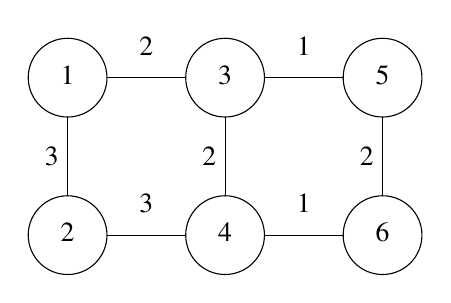
\begin{tikzpicture}
  %ノード1  
  \draw(4,2) circle (0.5)
  node[at={(4.0,2.0)}] {
    \begin{tabular}{c}
      1
    \end{tabular}
  };
  %ノード2  
  \draw(4,0) circle (0.5)
  node[at={(4.0,0.0)}] {
    \begin{tabular}{c}
      2
    \end{tabular}
  };
  %ノード3  
  \draw(6,2) circle (0.5)
  node[at={(6.0,2.0)}] {
    \begin{tabular}{c}
      3
    \end{tabular}
  };
  %ノード4  
  \draw(6,0) circle (0.5)
  node[at={(6.0,0.0)}] {
    \begin{tabular}{c}
      4
    \end{tabular}
  };
  %ノード5  
  \draw(8,2) circle (0.5)
  node[at={(8.0,2.0)}] {
    \begin{tabular}{c}
      5
    \end{tabular}
  };
  %ノード6  
  \draw(8,0) circle (0.5)
  node[at={(8.0,0.0)}] {
    \begin{tabular}{c}
      6
    \end{tabular}
  };
  \draw(4,0.5) --(4,1.5)
  node[at={(3.8,1.0)}] {3};
  \draw(6,0.5) --(6,1.5)
  node[at={(5.8,1.0)}] {2};
  \draw(8,0.5) --(8,1.5)
  node[at={(7.8,1.0)}] {2};
  \draw(4.5,0) --(5.5,0)
  node[at={(5.0,0.4)}] {3};
  \draw(4.5,2) --(5.5,2)
  node[at={(5.0,2.4)}] {2};
  \draw(6.5,0) --(7.5,0)
  node[at={(7.0,0.4)}] {1};
  \draw(6.5,2) --(7.5,2)
  node[at={(7.0,2.4)}] {1};
\end{tikzpicture}
}
\end{center}
%%%%%%%%%%%%%%%%%%%%%%%%%%%%%%

%%%%%%%%%%%%%%%%%%%%%%%%%%%%%%
\begin{exampleblock}{\code{graph.lp}}
\lstinputlisting[frame=none,numbers=none]{code/graph_example.lp} 
\end{exampleblock}
%%%%%%%%%%%%%%%%%%%%%%%%%%%%%%

\begin{itemize}
\item HCPの場合,距離を表すアトム\code{cost/3}は省略可.
\end{itemize}

\end{frame}
%%%%%%%%%%%%%%%%%%%%%%%%%%%%%%%%%%%%%%%%%%%%%%%%%%%%%%%%%%%%%%%%%%%
\begin{frame}{考案したハミルトン閉路問題の ASP 符号化}
%%%%%%%%%%%%%%%%%%%%%%%%%%%%%%%%%%%%%%%%%%%%%%%%%%%%%%%%%%%%%%%%%%%

\begin{block}{HCPの制約}
  HCP は与えられた無向グラフ$G= (V,E)$に対して,以下の2つの制約を満たす
  部分グラフ$G'= (V,E')$が存在するか判定する問題.
  \begin{itemize}
  \item $G'$の各頂点の次数が2 (\structure{次数制約})
  \item $G'$が連結 (\structure{連結制約})
  \end{itemize}
\end{block}

\begin{enumerate}
\item \alert{\textsf{undirected}符号化}
  \begin{itemize}
%  \item HCP の次数制約と連結制約を簡潔に表現した符号化.
  \item ASP の一貫性制約を用いて,\structure{連結制約を簡潔に表現}.
  \end{itemize}
\item \alert{\textsf{directed}符号化}
  \begin{itemize}
  \item \textsf{undirected}符号化をベースに,与えられた
    \structure{無向グラフを有向グラフ化}して解く符号化.
  \item SAT を用いた先行研究~{\scriptsize[Soh+,2014]}からヒントを得る.
  \end{itemize}
\item \alert{\textsf{acyclicity}符号化}
  \begin{itemize}
  \item \textsf{directed}符号化をベースに,連結制約を
    \structure{部分閉路を禁止する制約に置き換え}た符号化.
  \item ASP の\texttt{\#edge} 宣言を用いて,部分閉路禁止制約を簡潔に表現.
  \end{itemize}
\end{enumerate}
\end{frame}
%%%%%%%%%%%%%%%%%%%%%%%%%%%%%%%%%%%%%%%%%%%%%%%%%%%%%%%%%%%%%%%%%%%
\begin{frame}[shrink]{\code{undirected} 符号化}

\begin{exampleblock}{\code{undirected.lp}}
\lstinputlisting[numbers=none, frame=none]{code/hc1.lp}
\end{exampleblock}

\begin{itemize}
\item \code{(1)}: 各辺\code{edge(X,Y)}に対して,その辺がハミルト
      ン閉路に含まれるかどうかを意味するアトム\code{in(X,Y)}を導入する.
\item \code{(2)}: 次数制約.
      各頂点\code{node(X)}に対し,その次数が2に等しくなることを表す.
\item \code{(3)}--\code{(5)}: 頂点\code{X}が始点\code{s}から到達可能で
  あることを意味する補助アトム\code{reached(X)}を導入する.
\item \code{(6)}: 連結制約.各頂点\code{node(X)}が,
  始点から到達可能となることを表す.
\end{itemize}
\end{frame}
%%%%%%%%%%%%%%%%%%%%%%%%%%%%%%%%%%%%%%%%%%%%%%%%%%%%%%%%%%%%%%%%%%%
\begin{frame}[shrink]{ASP システム{\clingo}の実行例}
%%%%%%%%%%%%%%%%%%%%%%%%%%%%%%%%%%%%%%%%%%%%%%%%%%%%%%%%%%%%%%%%%%%
\begin{center}
\scalebox{0.8}[0.8]{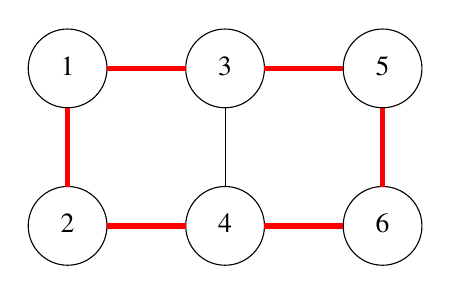
\begin{tikzpicture}
  %ノード1  
  \draw(4,2) circle (0.5)
  node[at={(4.0,2.0)}] {
    \begin{tabular}{c}
      1
    \end{tabular}
  };
  %ノード2  
  \draw(4,0) circle (0.5)
  node[at={(4.0,0.0)}] {
    \begin{tabular}{c}
      2
    \end{tabular}
  };
  %ノード3  
  \draw(6,2) circle (0.5)
  node[at={(6.0,2.0)}] {
    \begin{tabular}{c}
      3
    \end{tabular}
  };
  %ノード4  
  \draw(6,0) circle (0.5)
  node[at={(6.0,0.0)}] {
    \begin{tabular}{c}
      4
    \end{tabular}
  };
  %ノード5  
  \draw(8,2) circle (0.5)
  node[at={(8.0,2.0)}] {
    \begin{tabular}{c}
      5
    \end{tabular}
  };
  %ノード6  
  \draw(8,0) circle (0.5)
  node[at={(8.0,0.0)}] {
    \begin{tabular}{c}
      6
    \end{tabular}
  };
  \draw[red, line width=2pt](4,0.5) --(4,1.5)
  node[at={(3.8,1.0)}] {};
  \draw(6,0.5) --(6,1.5)
  node[at={(5.8,1.0)}] {};
  \draw[red, line width=2pt](8,0.5) --(8,1.5)
  node[at={(7.8,1.0)}] {};
  \draw[red, line width=2pt](4.5,0) --(5.5,0)
  node[at={(5.0,0.4)}] {};
  \draw[red, line width=2pt](4.5,2) --(5.5,2)
  node[at={(5.0,2.4)}] {};
  \draw[red, line width=2pt](6.5,0) --(7.5,0)
  node[at={(7.0,0.4)}] {};
  \draw[red, line width=2pt](6.5,2) --(7.5,2)
  node[at={(7.0,2.4)}] {};
\end{tikzpicture}
}
\end{center}

\begin{exampleblock}{}
\lstinputlisting[numbers=none,frame=none]{code/output.txt}
\end{exampleblock}

\end{frame}
%%%%%%%%%%%%%%%%%%%%%%%%%%%%%%%%%%%%%%%%%%%%%%%%%%%%%%%%%%%%%%%%%%%
\begin{frame}[shrink]{\code{directed} 符号化}
%%%%%%%%%%%%%%%%%%%%%%%%%%%%%%%%%%%%%%%%%%%%%%%%%%%%%%%%%%%%%%%%%%%

\begin{exampleblock}{\code{directed.lp}}
\lstinputlisting[numbers=none, frame=none]{code/hc2.lp}
\end{exampleblock}

\only<1>{
\begin{itemize}
\item \code{(1)}: 与えられた無向グラフの各辺 \code{edge(X,Y)} に対して,
  \alert{弧 \code{X}~$\rightarrow$~\code{Y}}を表す
  \code{in(X,Y)} と
  \alert{弧 \code{Y}~$\rightarrow$~\code{X}}を表す
  \code{in(Y,X)} の2個のアトムを導入し,
  2つの弧のうち,高々1個がハミルトン閉路に含まれることを表す.
\end{itemize}
}
\only<2>{
\begin{itemize}
\item \code{(2)}--\code{(3)}: 次数制約
  \begin{itemize}
  \item \code{(2)}: 各頂点\code{node(X)}の出次数が1に等しいことを表す.
  \item \code{(3)}: 各頂点\code{node(X)}の入次数が1に等しいことを表す.
  \end{itemize}
\item \code{(4)}--\code{(6)}: 連結制約は,\textsf{undirected}符号化と同じ.
\item \code{(7)}: 対称解を除去する制約
\end{itemize}
}
\end{frame}
%%%%%%%%%%%%%%%%%%%%%%%%%%%%%%%%%%%%%%%%%%%%%%%%%%%%%%%%%%%%%%%%%%%
\begin{frame}[shrink]{\code{acyclicity} 符号化}
%%%%%%%%%%%%%%%%%%%%%%%%%%%%%%%%%%%%%%%%%%%%%%%%%%%%%%%%%%%%%%%%%%%

\begin{exampleblock}{\code{acyclicity.lp}}
\lstinputlisting[numbers=none, frame=none]{code/hc3.lp}
\end{exampleblock}

\begin{itemize}
\item HCP の連結制約を\alert{部分閉路を禁止する制約}に置き換える.
\item \code{directed} 符号化との違いは,ルール \code{(4)} のみ.
\item \code{(4)}: \code{\#edge} 宣言を用いて,
  始点 \code{s} を含まない弧 \code{in(X,Y)} で構成される
  有向グラフが閉路を含まないことを保証する.
\item {\clingo}の \code{\#edge} 宣言は,
  ASP Modulo Theories 技術によって実装されている.
\end{itemize}
\end{frame}

%%%%%%%%%%%%%%%%%%%%%%%%%%%%%%%%%%%%%%%%%%%%%%%%%%%%%%%%%%%%%%%%%%%
\begin{frame}{実験概要}
%%%%%%%%%%%%%%%%%%%%%%%%%%%%%%%%%%%%%%%%%%%%%%%%%%%%%%%%%%%%%%%%%%%
\begin{block}{}\centering
  考案した ASP 符号化の有効性を評価するために実験を行った.
\end{block}
\vfill

\begin{exampleblock}{ベンチマーク問題}
  \begin{enumerate}
  \item \alert{ハミルトン閉路問題}
    \begin{itemize}
    \item FHCP ベンチマーク問題集 (計1,001問)
    \item 時間制限: 30分/問
    \end{itemize}
  \item 最短ハミルトン路問題
    \begin{itemize}
    \item 米国本土48州の隣接関係を表すグラフ,グリッドグラフ
    \item 時間制限: 3時間/問
    \end{itemize}
  \item コスト制約付きハミルトン路問題 (解の全列挙)
    \begin{itemize}
  \item 米国本土48州の隣接関係を表すグラフ
%    \item コスト制約の閾値を変化させた計10問
    \item 時間制限: 3時間/問
    \end{itemize}
    \end{enumerate}
\end{exampleblock}

\begin{itemize}
  \item \structure{ASP システム}: {\clingo}-5.5.0
  \item \structure{実験環境}: Mac OS, Intel Corei7 3.2GHz, 64GBメモリ
\end{itemize}

\end{frame}
%%%%%%%%%%%%%%%%%%%%%%%%%%%%%%%%%%%%%%%%%%%%%%%%%%%%%%%%%%%%%%%%%%%
\begin{frame}{HCP: ベンチマーク問題集}
%%%%%%%%%%%%%%%%%%%%%%%%%%%%%%%%%%%%%%%%%%%%%%%%%%%%%%%%%%%%%%%%%%%

\begin{block}{}\centering
Flinders Hamiltonian Cycle Project (FHCP)~\footnotemark[2] で
公開されている HCP インスタンス(全1,001問)を使用した.
\end{block}
\vfill
\begin{itemize}
\item FHCP Challenge 国際競技会(2015年--2016年)で使用
\item 頂点数は66個から9,528個 (平均は約3000個)
\item すべてハミルトン閉路が存在する(充足可能な)インスタンス
\item 代表的な TSP ソルバー \textsf{Concorde}, \textsf{LKH}, \textsf{SLH}
  のうち,2つ以上で解くことが難しいと判断された問題で構成されている.
\item 標準的な HCP ヒューリスティックスでは解くのが難しいように設計され
  ている.
\end{itemize}

\footnotetext[2]{https://sites.flinders.edu.au/flinders-hamiltonian-cycle-project/}
\end{frame}
%%%%%%%%%%%%%%%%%%%%%%%%%%%%%%%%%%%%%%%%%%%%%%%%%%%%%%%%%%%%%%%%%%%
\begin{frame}{HCP: 解けた問題数}
%%%%%%%%%%%%%%%%%%%%%%%%%%%%%%%%%%%%%%%%%%%%%%%%%%%%%%%%%%%%%%%%%%%

%%%%%%%%%%
\begin{table}[t]\scriptsize
  \centering
  %\tabcolsep = 0.8mm
  \renewcommand{\arraystretch}{1.2}
  \begin{tabular}{lr|rrr}
    問題サイズ & 問題数 & \textsf{undirected} & \textsf{directed} & \textsf{acyclicity}\\
   \hline
    $\:\:\:\:\:\,\, 0 \leq |V| < 1000$     & 171   & 156   & \alert{171}   & 156  \\ %
    $1000 \leq |V| < 2000$  & 165   & 120   & \alert{159}   & 121  \\
    $2000 \leq |V| < 3000$  & 177   & 125   & \alert{163}   & 80   \\
    $3000 \leq |V| < 4000$  & 185   & 104   & \alert{147}   & 48   \\
    $4000 \leq |V| < 5000$  & 128   & 92    & \alert{106}   & 30   \\
    $5000 \leq |V| < 6000$  & 80    & 63    & \alert{70}    & 21   \\
    $6000 \leq |V| < 7000$  & 55    & 39    & \alert{41}    & 20   \\
    $7000 \leq |V| < 8000$  & 28    & 12    & \alert{15}    & 4    \\
    $8000 \leq |V| < 9000$  & 10    & 2     & \alert{5}     & 1    \\
    $9000 \leq |V| < 10000$  & 2     & \alert{2}     & \alert{2}     & 1    \\
   \hline
    合計 & 1001 & 715   & \alert{879}   & 482  
  \end{tabular}
  \vskip .5em
%  \caption{ハミルトン閉路問題: 解けた問題数}
  \label{sat_table}
\end{table}
%label{sat_table}
%%%%%%%%%%

\begin{itemize}
\item \code{directed} 符号化が最も多い 879 問を解いた.
\item \code{directed} 符号化は,どの頂点数の範囲においても良い結果を示
  しており,その優位性が確認できる.
\end{itemize}
\end{frame}

%%%%%%%%%%%%%%%%%%%%%%%%%%%%%%%%%%%%%%%%%%%%%%%%%%%%%%%%%%%%%%%%%%%
\begin{frame}{HCP: カクタスプロット}
%%%%%%%%%%%%%%%%%%%%%%%%%%%%%%%%%%%%%%%%%%%%%%%%%%%%%%%%%%%%%%%%%%%

\begin{center}
  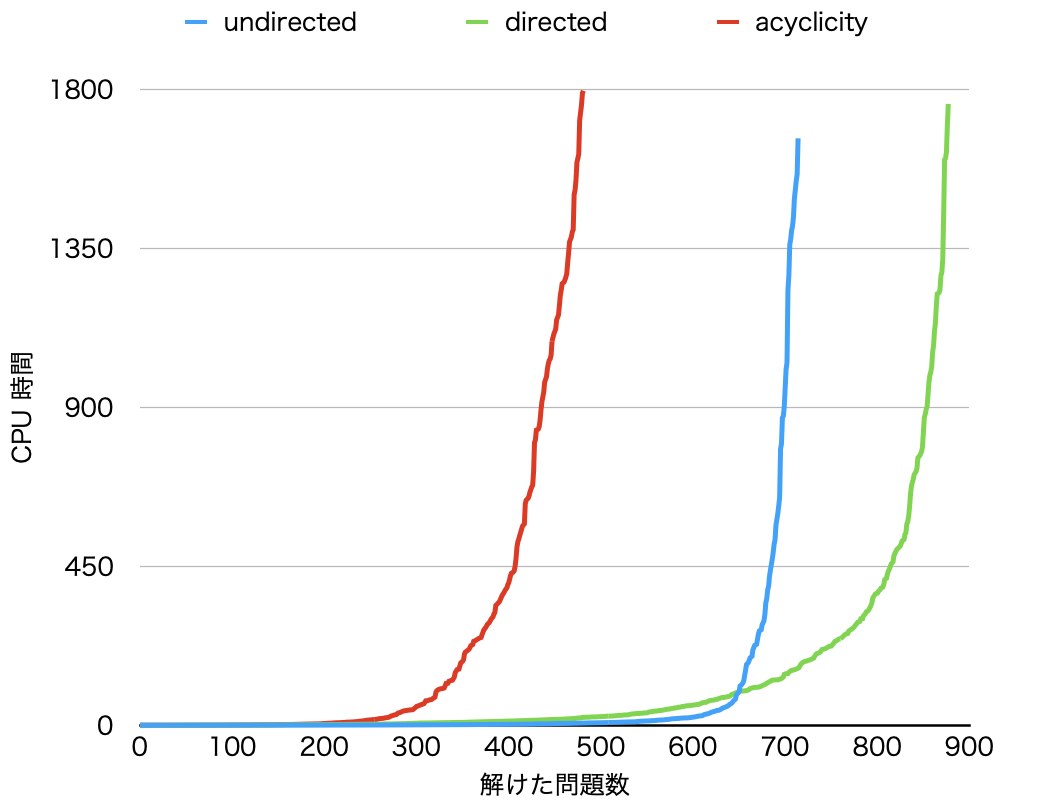
\includegraphics[width=0.7\linewidth]{fig/cactus.png}
\end{center}

\begin{itemize}
\item \code{directed} 符号化が,他の2つの符号化と比較して,
  より多くの問題を高速に解いていることがわかる.
\end{itemize}
\end{frame}

%%%%%%%%%%%%%%%%%%%%%%%%%%%%%%%%%%%%%%%%%%%%%%%%%%%%%%%%%%%%%%%%%%% 
\begin{frame}[shrink]{HCP: 解けた問題数の内訳}
%%%%%%%%%%%%%%%%%%%%%%%%%%%%%%%%%%%%%%%%%%%%%%%%%%%%%%%%%%%%%%%%%%% 
  
%%%%%%%%%%%%%%%%%%%%%%%%%%%%%%
\begin{center}
\scalebox{0.5}[0.5]{%\begin{tikzpicture}

%\end{tikzpicture}
}
% 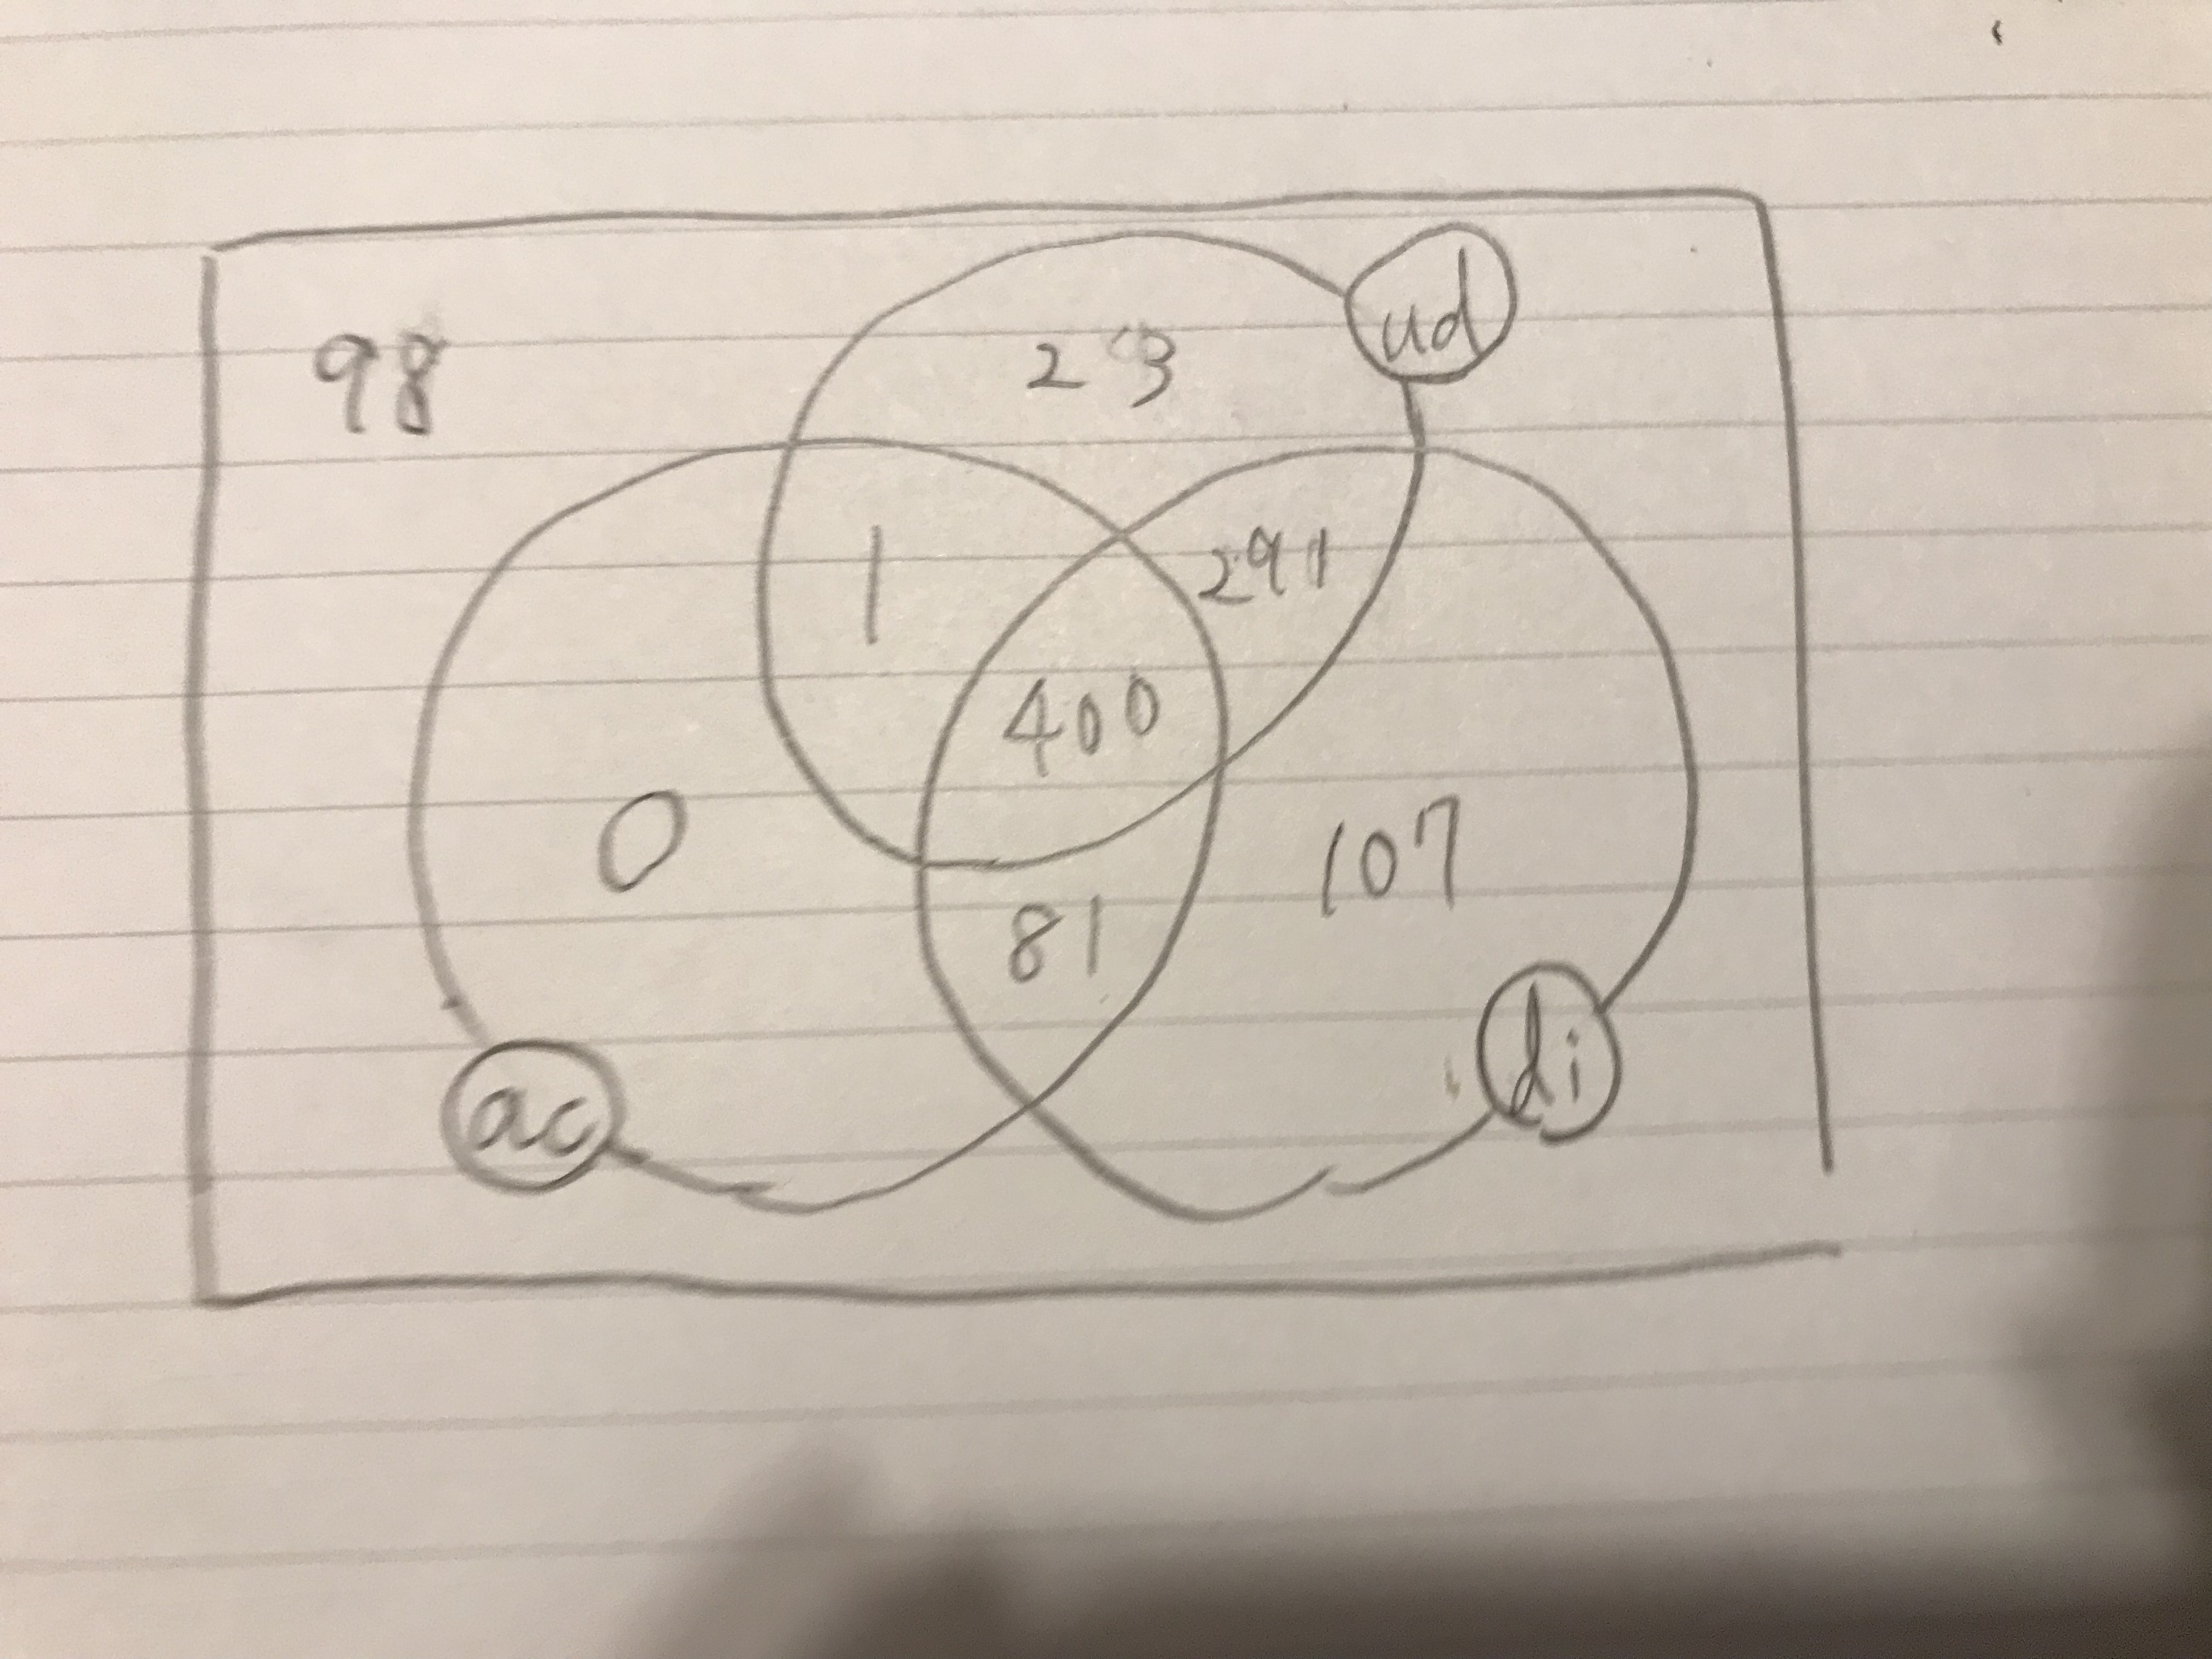
\includegraphics[width=0.5\linewidth]{fig/venn.jpeg}
\end{center}
%%%%%%%%%%%%%%%%%%%%%%%%%%%%%%
\vfill
\begin{itemize}
\item 全1,001問のうち,いずれかの符号化で解けた問題数は903問,
  どの符号化でも解けなかった問題数は98問であった.
\item \code{acyclicity} 符号化で解けた482問は,1問を除いて,
  \code{directed} 符号化でも解けている.
\item \code{undirected} と \code{directed} を比較すると,
  片方で解けて,もう片方で解けていない問題が一定数存在する.
\end{itemize}
\end{frame}
%%%%%%%%%%%%%%%%%%%%%%%%%%%%%%%%%%%%%%%%%%%%%%%%%%%%%%%%%%%%%%%%%%%
\begin{frame}{他のアプローチとの比較}
%%%%%%%%%%%%%%%%%%%%%%%%%%%%%%%%%%%%%%%%%%%%%%%%%%%%%%%%%%%%%%%%%%%
\begin{block}{}\centering
  FHCP Challenge 競技会(2015--2016)の上位5チームの成績~\footnotemark[3].
\end{block}
\vfill
\begin{tabular}[t]{clrc}
順位 & チーム & 問題数 & 手法 \\\hline
1 & INRIA, France & 985 & CPLEX \\
%\only<2>{ & \alert{ASP バーチャルベスト} & 903 & ASP \\}
\only<2>{ & \alert{ASP \code{directed} 符号化 (提案)} & 879 & ASP \\}
2 & IBM, United Kingdom & 614 & SAT \\
3 & King Saud University, Saudi Arabia & 488 & 不明 \\
4 & TU Darmstadt, Germany & 464 & 不明 \\
5 & Independent Researcher & 385 & 不明 \\\hline
\end{tabular}
\vfill

\begin{alertblock}<2>{}\centering
  提案手法は,ルール7個のASP符号化と汎用ソルバーの組合せで,
  \alert{実質2位に相当する成績}を示した.
\end{alertblock}

\footnotetext[3]{http://fhcp.edu.au/fhcpcs}
\end{frame}
%%%%%%%%%%%%%%%%%%%%%%%%%%%%%%%%%%%%%%%%%%%%%%%%%%%%%%%%%%%%%%%%%%%
\begin{frame}{まとめ}
%%%%%%%%%%%%%%%%%%%%%%%%%%%%%%%%%%%%%%%%%%%%%%%%%%%%%%%%%%%%%%%%%%%
% \begin{alertblock}{}\centering
% ASP を用いたハミルトン閉路問題の解法について述べた.
% \end{alertblock}
% \vfill

\begin{enumerate}
\item \structure{ハミルトン閉路問題を解く3種類の ASP 符号化を考案}
  \begin{itemize}
  \item ASP の \alert{ルール7個}程度で簡潔に表現できることを確認.
  \end{itemize}
\item \structure{FHCPベンチマーク問題集を用いた評価実験}
  \begin{itemize}
  \item \code{directed} 符号化が879問と最も多くの問題を解き,
    他の符号化と比較して,その優位性が確認できた.
  \item FHCP Challenge 競技会の上位ソルバーの成績と比較した結果,
    directed 符号化は\alert{実質2位}に相当する性能を示した.
  \end{itemize}
\item \structure{最短ハミルトン閉路問題,コスト制約付きハミルト
    ン閉路問題への拡張,および評価実験} (今回は省略)
\end{enumerate}

\begin{block}{今後の課題}
  \begin{itemize}
  \item 実験結果のより詳細な分析.\code{directed} 符号化が多くの問題を
    解けた理由等
  \item 緩和問題と CEGARを用いた解法~{\scriptsize[Soh+,2014]}の実装.
  \item 巡回セールスマン問題への拡張.
  \end{itemize}
\end{block}
\end{frame}
%%%%%%%%%%%%%%%%%%%%%%%%%%%%%%%%%%%%%%%%%%%%%%%%%%%%%%%%%%%%%%%%%%%
\appendix
%%%%%%%%%%%%%%%%%%%%%%%%%%%%%%%%%%%%%%%%%%%%%%%%%%%%%%%%%%%%%%%%%%% 
\begin{frame}{}
  \begin{center}\Huge
    Appendix
  \end{center}
\end{frame}
%%%%%%%%%%%%%%%%%%%%%%%%%%%%%%%%%%%%%%%%%%%%%%%%%%%%%%%%%%%%%%%%%%%
\begin{frame}{最短ハミルトン閉路問題への拡張}
%%%%%%%%%%%%%%%%%%%%%%%%%%%%%%%%%%%%%%%%%%%%%%%%%%%%%%%%%%%%%%%%%%%
\begin{exampleblock}{目的関数}
\lstinputlisting[frame=none, numbers=none]{code/obj_minimize.lp} 
\end{exampleblock}


\begin{itemize}
\item \textsf{undirected}, \textsf{directed}, \textsf{acyclicity}
  の各符号化に,上の目的関数を追加すればよい.
\item \textsf{undirected} の場合は,\code{(2)} のルールは不要.
\end{itemize}
\end{frame}
%%%%%%%%%%%%%%%%%%%%%%%%%%%%%%%%%%%%%%%%%%%%%%%%%%%%%%%%%%%%%%%%%%%
\begin{frame}{コスト制約付きハミルトン閉路問題への拡張}
%%%%%%%%%%%%%%%%%%%%%%%%%%%%%%%%%%%%%%%%%%%%%%%%%%%%%%%%%%%%%%%%%%%
\begin{exampleblock}{コスト制約}
\lstinputlisting[frame=none, numbers=none]{code/cost_constraint.lp}
\end{exampleblock}

\begin{itemize}
\item \textsf{undirected}, \textsf{directed}, \textsf{acyclicity}
  の各符号化に,上のコスト制約を追加すればよい.
\item 定数 \code{c} は閾値を表し,実際の値は実行に与えられる.
\item \textsf{undirected} の場合は,\code{(2)} のルールは不要.
\end{itemize}
\end{frame}
%%%%%%%%%%%%%%%%%%%%%%%%%%%%%%%%%%%%%%%%%%%%%%%%%%%%%%%%%%%%%%%%%%%
\begin{frame}{最短ハミルトン路問題の実験結果}
%%%%%%%%%%%%%%%%%%%%%%%%%%%%%%%%%%%%%%%%%%%%%%%%%%%%%%%%%%%%%%%%%%%
\begin{block}{}\centering
  各符号化で得られた目的関数の値を示す.    
\end{block}
  
\begin{center}
\begin{table}[htbp]
  \caption{実験結果2-1:trendy}
  \label{min_table_tr}
  \centering
  \begin{tabular}{|l|rrr|}
    \hline
    Instance&undirected&directed&acyclicity \\
    \hline
    grid5&50,656*&50,656*&50,656* \\
    grid6&68,656*&68,656*&68,656* \\
    grid7&91,822*&91,822*&91,822* \\
grid8&113,250&\textcolor{red}{112,916}&113,277 \\
grid9&\textcolor{red}{142,502}&143,326&143,660 \\
grid10rc&\textcolor{red}{172,703}&174,866&175,999 \\
grid11&\textcolor{red}{200,399}&204,456&200,638 \\
grid12&\textcolor{red}{231,278}&239,275&232,012 \\
grid13&\textcolor{red}{276,692}&276,926&276,899 \\
grid14&317,617&\textcolor{red}{317,144}&317,676 \\
grid15&\textcolor{red}{375,906}&376,809&376,210 \\
grid16&421,249&\textcolor{red}{419,737}&423,753 \\
US48&11,698*&11,698*&11,698* \\
    \hline
  \end{tabular}
\end{table}
%\label{min_table_tr}    
\end{center}

\begin{itemize}
\item 最適値と最良値の数は,
      \code{undirected} 符号化が5問で最も多い.
\end{itemize}
\end{frame}
%%%%%%%%%%%%%%%%%%%%%%%%%%%%%%%%%%%%%%%%%%%%%%%%%%%%%%%%%%%%%%%%%%%
\begin{frame}{コスト制約付きハミルトン路問題の実験結果}
%%%%%%%%%%%%%%%%%%%%%%%%%%%%%%%%%%%%%%%%%%%%%%%%%%%%%%%%%%%%%%%%%%%

\begin{block}{}\centering
  解の全列挙に要した CPU 時間(秒)を示す.
\end{block}

\begin{center}
  \scalebox{0.7}[0.7]{
    \begin{table*}[tb]\footnotesize
  \tabcolsep = 2mm
  %\renewcommand{\arraystretch}{1.0}
  \vskip .5em
  \centering
  \begin{tabular}{lr|rrr}
    \hline
    閾値(倍率)    &	解の総数 & \textsf{undirected} & \textsf{directed} & \textsf{acyclicity} \\
    \hline
    11698(1.00)   &	1      &\textbf{2.979} & 7.531 & 4.586	\\
    11814(1.01)   &	8      &5.587  & 15.322	& \textbf{5.250}	\\
    11931(1.02)   &	28     &\textbf{3.243}& 18.600	& 3.578	\\
    12282(1.05)   &	388    &10.003&19.818	& \textbf{6.296}	\\
    12867(1.10)   &	16,180  &16.548& 28.555	& \textbf{9.764}\\
    14037(1.20)   &	939,209 &48.262       &40.717	& \textbf{26.837}\\
    15207(1.30)   &	4,525,541&88.172      &55.276	& \textbf{42.037}\\
    16377(1.40)   &	6,702,964&99.154       &47.647	& \textbf{40.640}	\\
    17547(1.50)   &	6,876,526&95.390       &45.265	& \textbf{38.411}	\\
    18716(1.60)   &	6,876,928&98.937       &49.138	& \textbf{40.748}	\\
    \hline
    平均CPU時間 &   & 46.8275 & 32.7869  & \textbf{21.8147}\\\hline
%    Best    &   & 2 & 0 & \textbf{8} \\ \hline
  \end{tabular}
  \vskip .5em
  \caption{コスト制約付きハミルトン路問題: 解の全列挙に要した CPU 時間}
  \label{cost_table}
\end{table*}

  }
\end{center}

%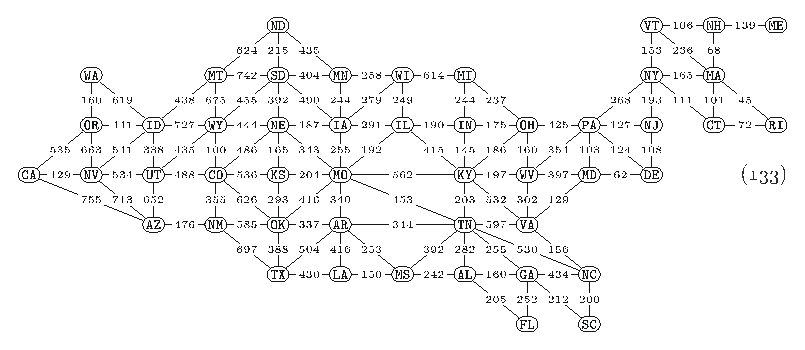
\includegraphics[width=0.7\linewidth]{fig/taocp_vol4fasc1b_p52_eq133.pdf}

\begin{itemize}
\item \code{acyclicity} 符号化が,より多くの問題を
  高速に解き,平均 CPU 時間も最も短かった.
\end{itemize}  
\end{frame}
%%%%%%%%%%%%%%%%%%%%%%%%%%%%%%%%%%%%%%%%%%%%%%%%%%%%%%%%%%%%%%%%%%%
% \begin{frame}[noframenumbering]{参考文献}
% \bibliographystyle{jplain} % 参考文献スタイル
% \bibliography{aisat,bachelor}    % 参考文献リスト
% \end{frame}
%%%%%%%%%%%%%%%%%%%%%%%%%%%%%%%%%%%%%%%%%%%%%%%%%%%%%%%%%%%%%%%%%%%

\end{document}

%%% Local Variables:
%%% mode: japanese-latex
%%% TeX-master: t
%%% End:
